%=========================================
% 	   Sicherheit						 =
%=========================================
\section{Sicherheitsaspekte}

Jede Anwendung muss eine sichere Umgebung zur Verfügung stellen. Vor allem 
Webanwendungen bedürfen oft besonderer Sicherheit, da unsichere
Implementierungen mit einigen Tricks umgangen werden können und Nutzer dadurch 
Zugriff auf Daten erhalten können, welche nicht für sie bestimmt sind. Einige 
Fragen müssen durchdacht werden, um eine nachhaltige Implementierung der 
Sicherheitsmechanismen zu gewährleisten:

\begin{itemize}
\item Wie werden Authentifizierung und Authorisierung sichergestellt?
\item Müssen beim Austausch des / der Server die Sicherheitsmechanismen neu implementiert und / oder die
	  Sicherheitseinstellungen neu konfiguriert werden?
\item An welchen Stellen der Anwendung werden sensible Daten übertragen und bedürfen kryptografischer 	      
      Verschlüsselung?
\end{itemize} 

Dieser Abschnitt zeigt, wie wir das Spring Framework nutzen, um eine sichere 
Umgebung und damit auch alle damit in Verbindung stehenden Sicherheitsanliegen 
gewährleisten.

\subsection{Spring Security Module}
\label{subsec:spring_security}

Das Spring Framework stellt den Service Spring Security zur Verfügung, welcher grundsätzlich genutzt 
werden kann, um alle oben genannten Problemstellungen zu lösen. Insgesamt stellt Spring Security folgende 
elf Module zur Implementierung von Sicherheitsmechanismen bereit:

\begin{table}[hbt]
 \caption[Spring Security Module, Quelle: Walls (2011), S. 246]{Spring Security Module \cite{walls:2011}}
  \begin{tabular}{lp{11cm}}
    \toprule 
    \textbf{Modul} & \textbf{Beschreibung} \\
    \hline
    ACL & Kapselt den Zugriff auf Geschäftsobjekte mittels Zugriffssteuerungslisten \\
    %------------------------------------------------------------------------------------------
    Aspects & Untestützt die Verwendung einer AspectJ-basierten Implementierung anstelle des Spring AOP Standards im Rahmen von Spring Security. \\
	%------------------------------------------------------------------------------------------
	CAS Client Support & Bietet eine Single Sign-on Authentifizierung (\grqq{} Einmalanmeldung\grqq{}), die mittels der Central Authentication Service (CAS) Technik umgesetzt wird. \\
	%------------------------------------------------------------------------------------------
	Configuration & Unterstützt die Konfiguration von Spring Security via Java und XML 
	(Java wird seit Spring Security 3.2. unterstützt) \\
	%------------------------------------------------------------------------------------------
	Core & Liefert die essentielle Spring Security Bibliothek \\
	%------------------------------------------------------------------------------------------
	Cryptography & Bietet Methoden zur Verschlüsselung und Passwortcodierung \\
	%------------------------------------------------------------------------------------------
	LDAP & Unterstützt eine LDAP-basierte Authetifizierung \\
	%------------------------------------------------------------------------------------------
	OpenID & Unterstüzt eine zentrale Authentifizierung mittels OpenID. \\
	%------------------------------------------------------------------------------------------
	Remoting & Sorgt für die Integration von verteilten, auf Spring basierenden Systemen. \\
	%------------------------------------------------------------------------------------------
	Tag Library & Die Spring Security JSP Tag Bibliothek. \\
	%------------------------------------------------------------------------------------------
	Web & Bietet eine, auf dem Spring Security \textit{Filter} basierende Technik, zur Unterstützung von Web-Sicherheitsaspekten. \\
	\bottomrule
  \end{tabular}
\end{table}

Normalerweise werden nicht alle Module benötigt. Auch bei uns werden nur die Module Core, 
Configuration und Web eingesetzt. Der in einem vorherigen Kapitel vorgestellte Service Maven wird an 
dieser Stelle eingesetzt, um sämtliche benötigte Module, welche als .jar Dateien geliefert werden, zu 
importieren.

\subsection{Implementierung und Funktionsweise}

Um Spring Security aktiv in der Anwendung nutzen zu können muss als erstes eine springSecurityFilterChain 
Klasse implementiert werden. Wie der Name der Klasse schon sagt, handelt es sich dabei um einen Filter, der 
jegliche ankommende Webanfragen durch alle implementierten Sicherheitsmechanismen laufen lässt, sozusagen 
verkettet, und den Einsatz von Spring Security so erst ermöglicht. Abbildung \ref{fig:user_privileges} stellt den 
grudsätzlichen Ablauf einer Anfrage und deren Filterung durch Sicherheitsmechanismen dar.

\begin{figure}
    \centering
    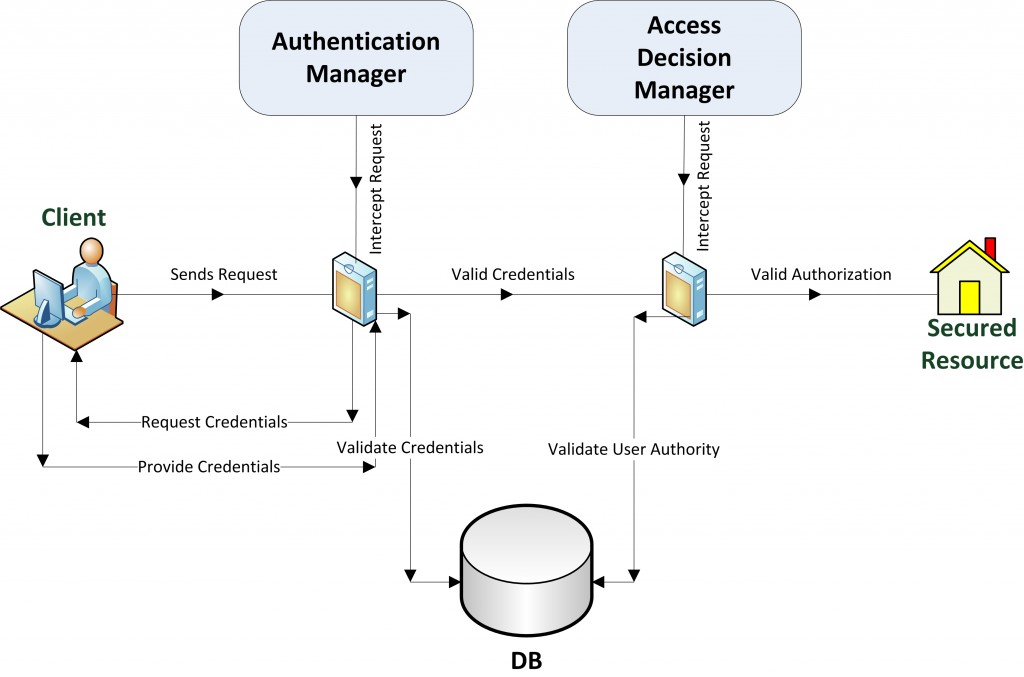
\includegraphics[width=0.85\textwidth]{Graphics/security/user_privileges}
    \caption[Authentifizierung und Validierung der Privilegien eines Nutzers, Quelle: \cite{javabook:sec}]{Authentifizierung und Validierung der Privilegien eines Nutzers \cite{javabook:sec}}
   \label{fig:user_privileges}
\end{figure}

Stellt ein Client nun eine Anfrage an eine Ressource, wird diese erst durch einen implementierten 
Authentication-Manager gefiltert. Die verschiedenen Unterfilter werden durch Authentication-Provider 
realisiert. Der Authentication-Provider prüft die beim Login eingegebenen Daten auf ihre Richtigkeit. 
Sind die Daten nicht im Code verankert und in einer Datenbank gespeichert, wird hier zusätzlich ein 
Jdbc-user-service benötigt, welcher die nötigen SQL-Anfragen zum Abgleichen der Nutzerdaten als 
Parameter erwartet. Hat der Abgleich mit der Datenbank stattgefunden und die Daten waren korrekt, wird 
die Anfrage weitergeleitet. In Abbildung \ref{fig:user_privileges} wird der folgende Prozess durch den Access Decision 
Manager dargestellt. Dieser ist in unserer konkreten Anwendung nicht implementiert, jedoch findet der 
Authorisierungsprozess hier -mittels Datenbankabfrage- trotzdem statt. An dieser Stelle muss überprüft werden, ob der Nutzer die 
nötigen Privilegien besitzt, um eine gewisse Seite aufrufen zu dürfen. Dieser Abgleich wird ebenfalls 
mit in der Datenbank gespeicherten Daten durchgeführt. An dieser Stelle gibt es folgende verschiedene 
Privilegien, die Spring Security zur Authorisierung zur Verfügung stellt: \newpage

\begin{table}[hbt]
 \caption[Die verschiedenen von Spring zur Verfügung gestellten Privilegien, Quelle: Walls (2011), S. 262]{Die verschiedenen von Spring zur Verfügung gestellten Privilegien \cite{walls:2011}}
  \begin{tabular}{lp{9.5cm}}
    \toprule 
    \textbf{Privileg} & \textbf{Beschreibung} \\
    \hline
    \texttt{hasRole([role])} & Gibt an, ob der aktuelle Benutzer die spezifizierte Rolle innehat \\
    %------------------------------------------------------------------------------------------
    \texttt{hasAnyRole([role1,role2])} & Gibt an, ob der aktuelle Benutzer eine der angegebenen Rollen innehat \\
	%------------------------------------------------------------------------------------------
	\texttt{principal} & Erlaubt direkten Zugriff auf den aktuellen Benutzer \\
	%------------------------------------------------------------------------------------------
	\texttt{authentication} & Erlaubt direkten Zugriff auf das aktuelle \texttt{Authentication} Objekt \\
	%------------------------------------------------------------------------------------------
	\texttt{permitAll} & Erlaubt einen uneingeschränkten Zugriff auf eine Ressource \\
	%------------------------------------------------------------------------------------------
	\texttt{denyAll} & Verweigert den Zugriff auf eine Ressource \\
	%------------------------------------------------------------------------------------------
	\texttt{isAnonymous()} & Gibt an, ob es sich bei dem aktuellen Benutzer um einen anonymen Benutzer handelt \\
	%------------------------------------------------------------------------------------------
	\texttt{isRememberMe()} & Gibt an, ob der aktuelle Benutzer ein sogenannter \grqq{} remember-me user\glqq ist, also bereits zu einem früheren Zeitpunkt authentifiziert wurde. \\
	%------------------------------------------------------------------------------------------
	\texttt{isAuthenticated()} & Gibt an, ob der aktuelle Benutzer authentifiziert ist. \\
	%------------------------------------------------------------------------------------------
	\texttt{isFullyAuthenticated()} & Gibt, an ob der aktuelle Benutzer authentifziert ist und die \grqq{} remember-me\grqq{} aktiviert hat \\
	\bottomrule
  \end{tabular}
\end{table} 
\bigskip
Wird auch dieser Abgleich erfolgreich durchgeführt, erhält der Nutzer Zugriff auf die Ressource. Das 
folgende Codesegment veranschaulicht unsere Implementierung, dieser Sicherheitsmechanismen: \\

\lstinputlisting [style=XML]{Snippets/security.xml}

Das durch den \texttt{AuthenticationManager} gekennzeichnete Codesegment zeigt die Implementierung des 
Validierungsprozesses der Logindaten.
Anhand des zweiten Abschnitts des Codesegments lässt sich erkennen, dass in unserer Anwendung z.B. die 
Startseite und die Seite zum Erstellen eines neuen Accounts von jedem Nutzer aufgerufen werden darf, 
da das \texttt{access} Attribut hier auf \texttt{permitAll} gesetzt wurde. Das Anzeigen der Tweets benötigt 
jedoch erst eine Authentifizierung, da der access Parameter den Wert \texttt{isAuthenticated()} 
annimmt. Natürlich könnten hier auch spezielle Bereiche für Administratoren eingerichtet werden. Das 
access Attribut müsste dort lediglich dementsprechend parametrisiert und die Autorität in der 
Datenbank hinterlegt werden.

\subsection{Verschlüsselung sensibler Daten}\label{subsec:secure_login}

Die vorherigen Abschnitte haben gezeigt, dass Spring Security in jeder Situation eine Lösung für die 
geforderte Problemstellung liefert. Auch im Bezug auf das Verschlüsseln von sensiblen Daten wie 
Passwörtern stellt das Modul eine einfache Lösung bereit. Da in unserer Anwendung das Anlegen von 
Accounts möglich sein soll und Passwörter aus Sicherheitsgründen nicht im Volltext in der Datenbank 
abgelegt werden dürfen, wird hier eine angemessene Verschlüsselungsmethode benötigt. Diese 
Verschlüsselung wird durch eine von Spring bereitgestellte passwordEncoder Klasse realisiert. Diese 
ist in der Lage, die eingegebenen Passwörter mithilfe folgender Algorithmen zu verschlüsseln:

\begin{enumerate}
  \item \textit{Bcrypt}: Eine auf dem Blowfish-Algorithmus basierende Funktion
  \item \textit{SHA}: Ein Verschlüsselungsalgorithmus der SHA-1 Familie
  \item \textit{SHA-256}: Ein Verschlüsselungsalgorithmus der SHA-2 Familie
  \item \textit{Md4}: Eine auf 32-Bit Systemen effektive Hashfunktion welche in 128-Bit verschlüsselt
  \item \textit{Md5}: Eine nicht mehr als sicher geltende Hashfunktion, die ebenfalls einen 128-Bit- 	Hashwert erzeugt
\end{enumerate}

Wir haben uns an dieser Stelle für die Verschlüsselung der Passwörter mittels der SHA-256 Hashfunktion 
entschieden, da diese, im Gegensatz zu den meisten anderen oben genannten Funktionen, einen 256-Bit-
Hashwert erzeugt, immer noch als stabil gilt und wir im Laufe des Studiums bisher nur mit den SHA-
Hashfunktionen in Kontakt gekommen sind. \\
Das Einbinden der \texttt{passwordEncoder} Klasse findet ebenfalls im Authentication-manager Abschnitt statt 
und erfordert nur wenige Zeilen: \\

\lstinputlisting [style=XML]{Snippets/security_auth_provider.xml} \newpage

Hierzu wird ein weiterer Authentication-Provider Abschnitt erzeugt, in dem sowohl die Datenbank als 
auch der \texttt{passwordEncoder} und die Art des Hashes als Parameter übergeben werden. Des weiteren muss die 
Klasse selbst eingebunden werden: \\

\lstinputlisting [style=XML]{Snippets/security_password_encoder.xml}
\bigskip 
Die von einem Nutzer eingegebenen Passwörter werden dann mittels SHA-256 verschlüsselt und in der 
Datenbank hinterlegt. \\
Abschließend bleibt zu sagen, dass die meisten von uns genutzten Klassen und in diesem Kapitel 
erläuterten Methoden nur eine Option darstellen, um jeweilige Problemstellungen zu lösen. Spring
Security ist ein mächtiger Service, der für jede Situation und Umgebung die nötigen Vorraussetzungen 
liefert, sichere und serverunabhängige Anwendungen zu schreiben. Des weiteren müssen von Spring-
Security bereitgestellte Klassen nicht zwangsläufig verwendet werden. Zum Beispiel wäre es möglich, 
einen eigenen Filter zu implementieren und dabei auf die \texttt{springSecurityFilterChain} Klasse zu 
verzichten.









